\documentclass{beamer}
%\usepackage[urlcolor=blue]{hyperref}
\definecolor{links}{HTML}{2A1B81}
\hypersetup{colorlinks,linkcolor=,urlcolor=blue}
\usepackage[utf8]{inputenc}
\usepackage[spanish]{babel}
\usepackage{graphicx}
\usepackage{booktabs}
\usepackage{ragged2e}
\usepackage{xcolor}
\definecolor{LightGray}{gray}{0.975}

\usepackage{tikz}
\usetikzlibrary{arrows,shapes}

\usepackage{algorithm}
\usepackage{algorithmic}

%\usetheme{Warsaw}
\usefonttheme{serif} 

\title[Chapter 1]{Database Administration: The Complete Guide to Practices and Procedures, $2^{nd}$  Edition.}
\subtitle{Chapter 1: What is a DBA?}
\author{Craig Mullins}
\date{\today}

\setbeamertemplate{navigation symbols}{}%remove navigation symbols

\defbeamertemplate*{footline}{shadow theme}
{%
  \leavevmode%
  \hbox{\begin{beamercolorbox}[wd=.5\paperwidth,ht=2.5ex,dp=1.125ex,leftskip=.3cm plus1fil,rightskip=.3cm]{author in head/foot}%
    \usebeamerfont{author in head/foot} Database Administration \hfill \insertshorttitle
  \end{beamercolorbox}%
  \begin{beamercolorbox}[wd=.5\paperwidth,ht=2.5ex,dp=1.125ex,leftskip=.3cm,rightskip=.3cm plus1fil]{title in head/foot}%
    \usebeamerfont{title in head/foot} \hfill \insertframenumber\,/\,\inserttotalframenumber%
  \end{beamercolorbox}}%
  \vskip0pt%
}

\AtBeginSection[]
{
     \begin{frame}<beamer>
     \frametitle{Plan}
     \tableofcontents[currentsection]
     \end{frame}
}

\newcommand{\toRight}[1]{
    \begin{FlushRight}
        {\tiny #1}
    \end{FlushRight}
} % Align to right

\begin{document}

\frame{\titlepage}

\begin{frame}{Database Administration: The Complete Guide to Practices and Procedures.}
    \centering
    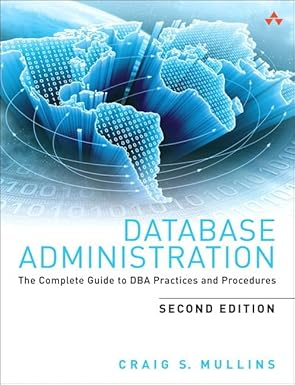
\includegraphics[width=0.3\textwidth]{figures/book_cover.jpg} \\
    \vspace{5mm}
    {
        \tiny
        Content has been extracted from \textit{Database Administration: The Complete Guide to Practices and Procedures.}, Second Edition, by Craig S. Mullin. Addison-Wesley Professional. 2012.\\
        Visit \url{https://www.craigsmullins.com/books.htm}.\\
    }
\end{frame}

\section{Conceptos Básicos}

\begin{frame}{Qué es una base de datos?}
    \begin{itemize}
        \item Una base de datos es un almacén organizado de datos en el que los datos son accesibles por elementos de datos con nombre. 
        \item Un DBMS es un software que permite a los usuarios finales o programadores de aplicaciones compartir datos.
        \item Proporciona un método sistemático para crear, actualizar, recuperar y almacenar información en una base de datos.
    \end{itemize}
    \toRight{Appendix 1, “Database Concepts and Fundamentals.”}
\end{frame}

\begin{frame}{Qué es una base de datos?}
    \begin{itemize}
        \item Los DBMS también son generalmente responsables de la integridad de los datos, la seguridad de los datos, el control y la optimización del acceso a los datos, la reversión automatizada, el reinicio y la recuperación. 
        \item En términos simples, puede pensar en una base de datos como una carpeta de archivos. Puede pensar en el archivador que contiene los archivos junto con las etiquetas de archivo como DBMS.
    \end{itemize}
    \toRight{Appendix 1, “Database Concepts and Fundamentals.”}
\end{frame}

\begin{frame}{Funciones del DBMS}
    \begin{itemize}
        \item Mantener la integridad de los datos.
        \item Garantizar la seguridad de los datos.
        \item Optimizar el acceso a los datos.
        \item Proveer reversión automatizada, reinicio y recuperación.
    \end{itemize}
\end{frame}

\begin{frame}{\_}
    \begin{tabular}{c}
        DBMS vs Database \\
        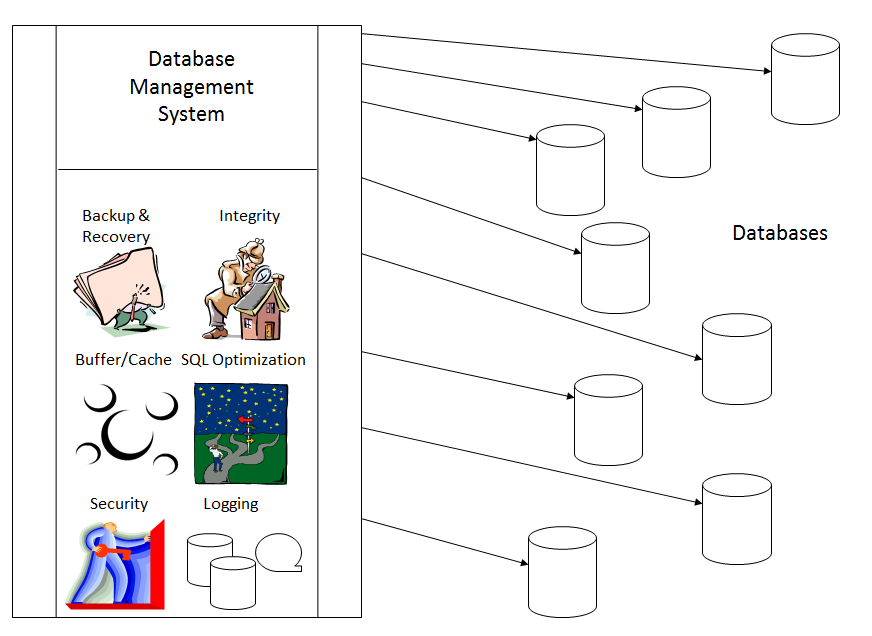
\includegraphics[width=0.9\textwidth]{figures/dbms_vs_database.png}
    \end{tabular}
    \toRight{\url{http://thedatabasesite.com/page100.html}}
\end{frame}

\section{Porqué aprender Administración de Bases de Datos?}

\begin{frame}{Porqué ser un DBA?}
    \begin{itemize}
        \item Diseñar y mantener las bases de datos de una empresa.
        \item Estar en el centro de los negocios.
        \item Aprender sobre nuevas tecnologías.
        \begin{itemize}
            \item Además de tener la oportunidad de aprender sobre muchas facetas de los negocios y cómo las empresas utilizan los datos.
        \end{itemize}
    \end{itemize}
\end{frame}

\begin{frame}{Qué hace a un buen DBA?}
    \begin{itemize}
        \item Solucionador de problemas.
        \item Disfruta de los desafíos.
        \item Aprendizaje constante.
        \item Puede trabajar solo o en equipo.
        \item Experiencia como programador.
    \end{itemize}
\end{frame}

\begin{frame}{Generalmente los DBAs obtienen buena remuneración por su trabajo...}
    \begin{itemize}
        \item According to a salary study conducted by Global Knowledge and TechRepublic the average DBA salary is \$78,468, while their managers average \$87,261. 
        \begin{itemize}
            \item For full-time employees functioning as a DBA, the mean salary ranges in the high \$80 thousands
        \end{itemize}

        \item According to the Dice 2010-11 Tech Salary Survey, Oracle experience is requested in more than 15,000 job postings on any given day. 
        \begin{itemize}
            \item Demand for Oracle skills is up 57\% year over year, and the national average salary for technology professionals with experience in Oracle Database is \$90,914. 
        \end{itemize}

        \item The BLS (May 2010) reports that the median annual wage of database administrators was \$73,490 and the mean annual wage was \$75,730. 
    \end{itemize}
\end{frame}

\begin{frame}{Generalmente los DBAs obtienen buena remuneración por su trabajo...}
    \noindent 
    \begin{minipage}{0.45\textwidth}
        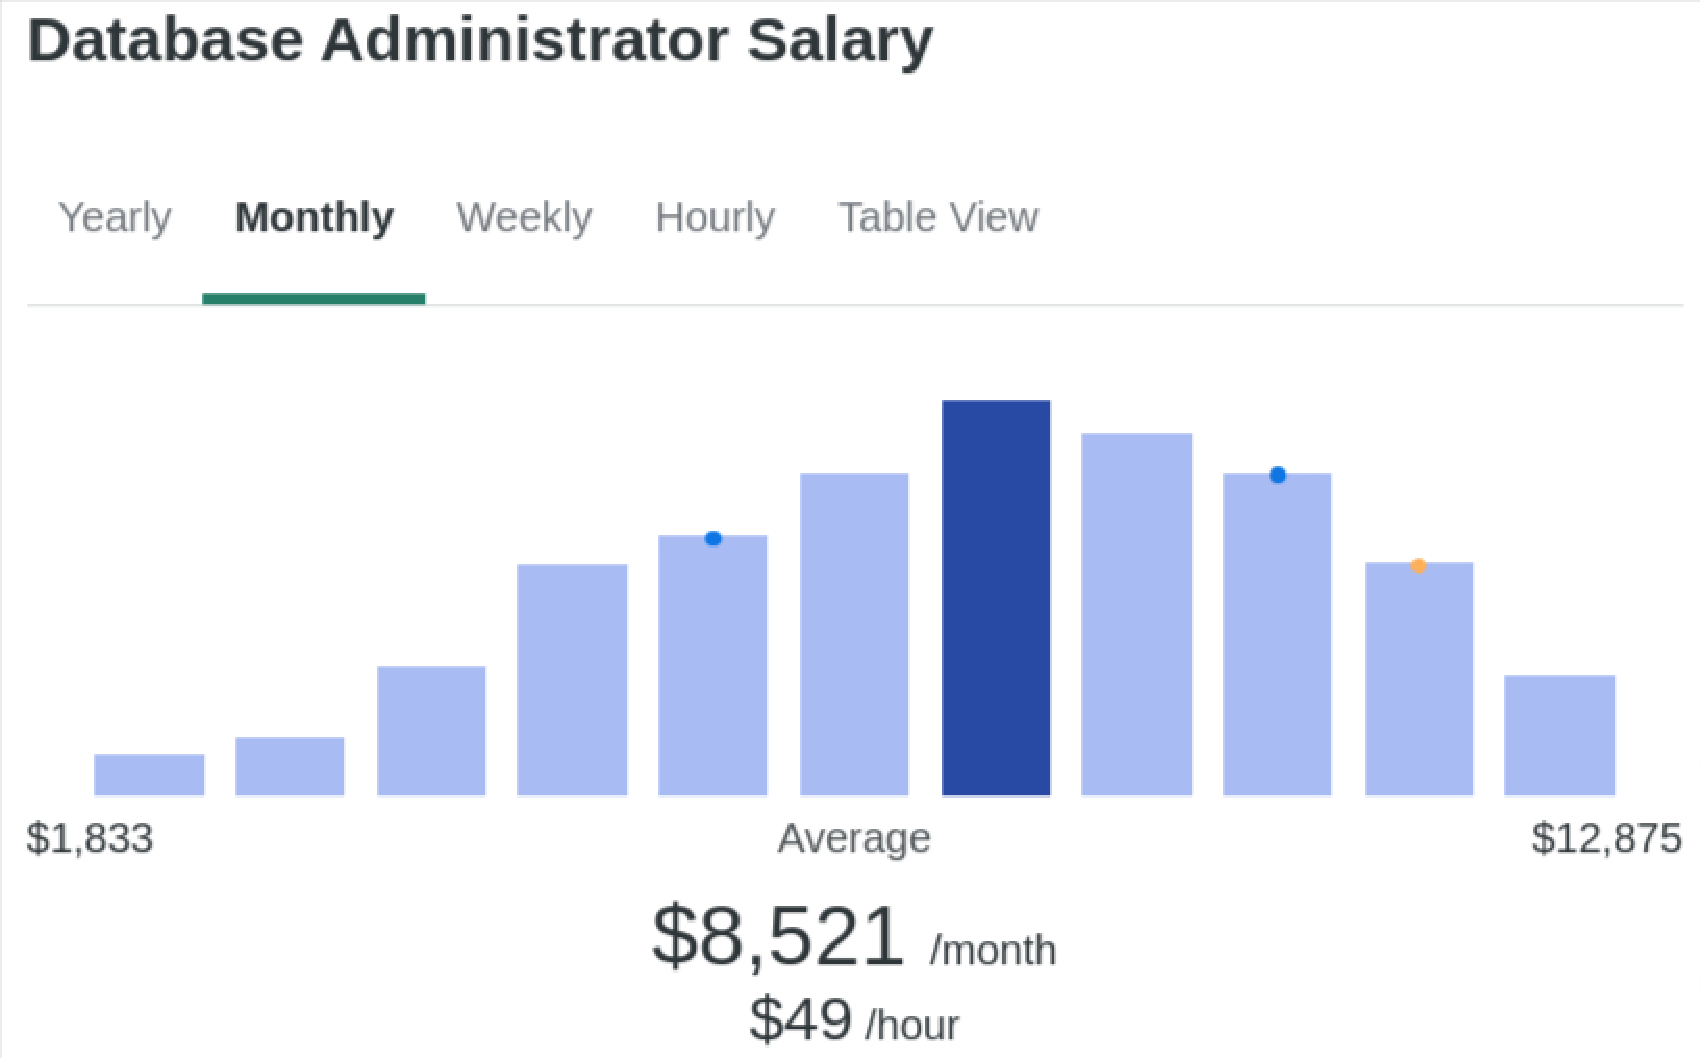
\includegraphics[width=\textwidth]{figures/dba_salary_plot}
    \end{minipage}
    \hspace{0.05\textwidth}
    \begin{minipage}{0.45\textwidth}
        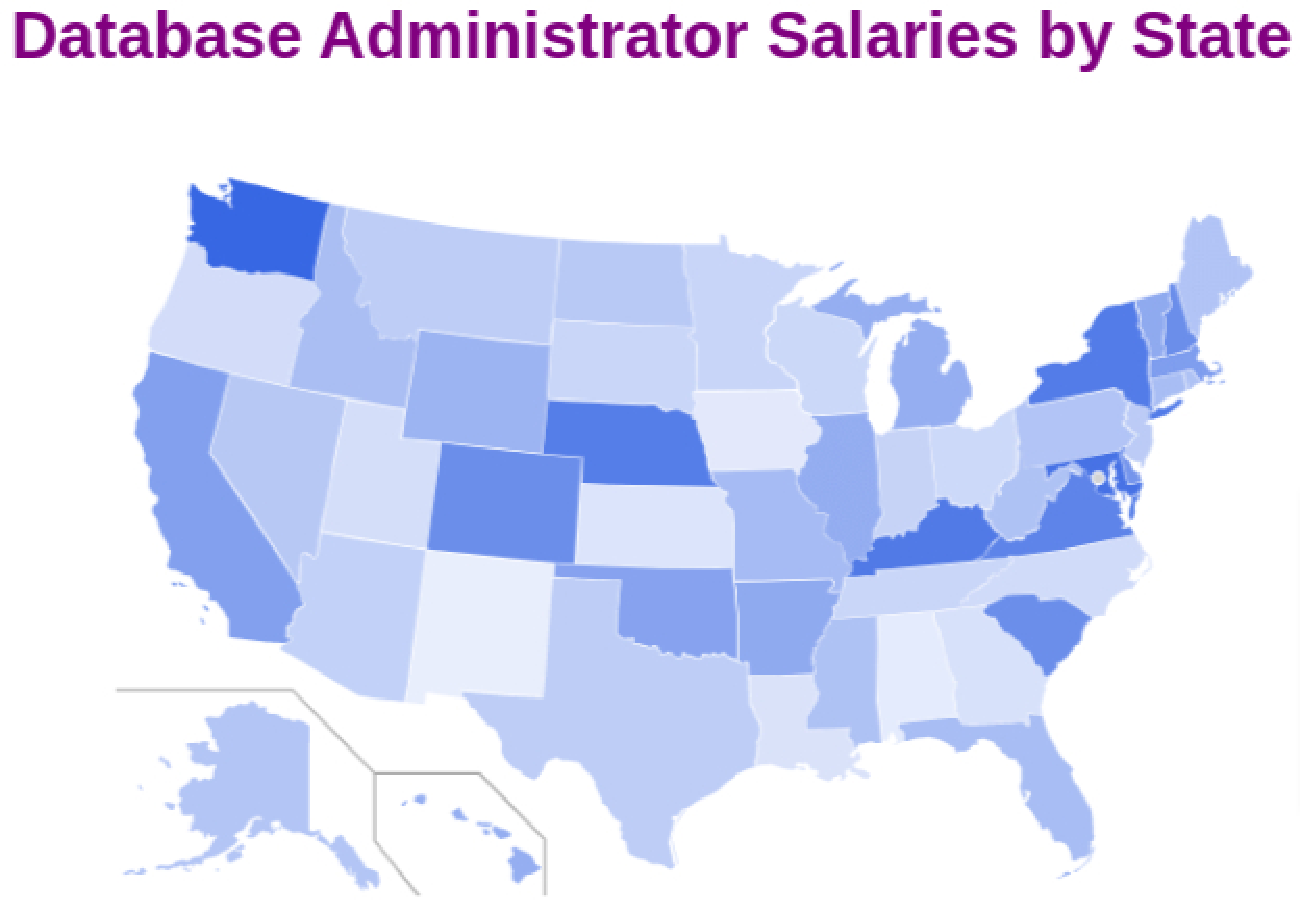
\includegraphics[width=0.9\textwidth]{figures/dba_salary_map}
    \end{minipage}%
    \vspace{5mm}
    Recursos adicionales:
    \begin{enumerate}
        \item \href{https://www.cs.ucr.edu/~acald013/public/Javeriana/DBA_Salary.html}{Estadísticas actuales} en US, Europa, Latinoamérica y Colombia.
        \item Diferentes \href{https://www.cs.ucr.edu/~acald013/public/Javeriana/Certifications.html}{tipos de certificaciones.}
    \end{enumerate}

\end{frame}

\begin{frame}{Desventajas de ser un DBA...}
    \begin{itemize}
        \item Los DBA están bien pagados, son altamente empleables, poseen trabajos desafiantes y es probable que participen en los proyectos más visibles e importantes. Pero...
        \item Se espera que los administradores de bases de datos sepan todo, no solo sobre la tecnología de bases de datos, sino sobre cualquier cosa conectada a ella. 
        \item Los DBA casi nunca trabajan días de 8 horas, sino que trabajan largas jornadas con muchas horas extras, especialmente cuando el rendimiento está sufriendo o los proyectos de desarrollo están retrasados. 
    \end{itemize}
\end{frame}


\begin{frame}{Desventajas de ser un DBA...}
    \begin{itemize}
        \item Según los analistas de la industria, el DBA promedio trabaja más de 50 horas por semana.
        \item Los administradores de bases de datos con frecuencia tienen que trabajar los fines de semana y días festivos para mantener las bases de datos durante las horas de menor actividad.
    \end{itemize}
\end{frame}

\begin{frame}{The Management Discipline of Database Administration}
    \begin{itemize}
        \item Un DBA es el técnico de información responsable de garantizar la funcionalidad operativa continua y la eficiencia de las bases de datos de una organización y las aplicaciones que acceden a esas bases de datos.
    \end{itemize}
    
    \toRight{\url{http://datatechnologytoday.wordpress.com/2011/02/27/dba-as-a-management-discipline/}}
\end{frame}

\section{Roles y Responsabilidades}

\begin{frame}{Roles y Responsabilidades}
    \begin{tabular}{c}
        Database, Data, and System Administration \\
        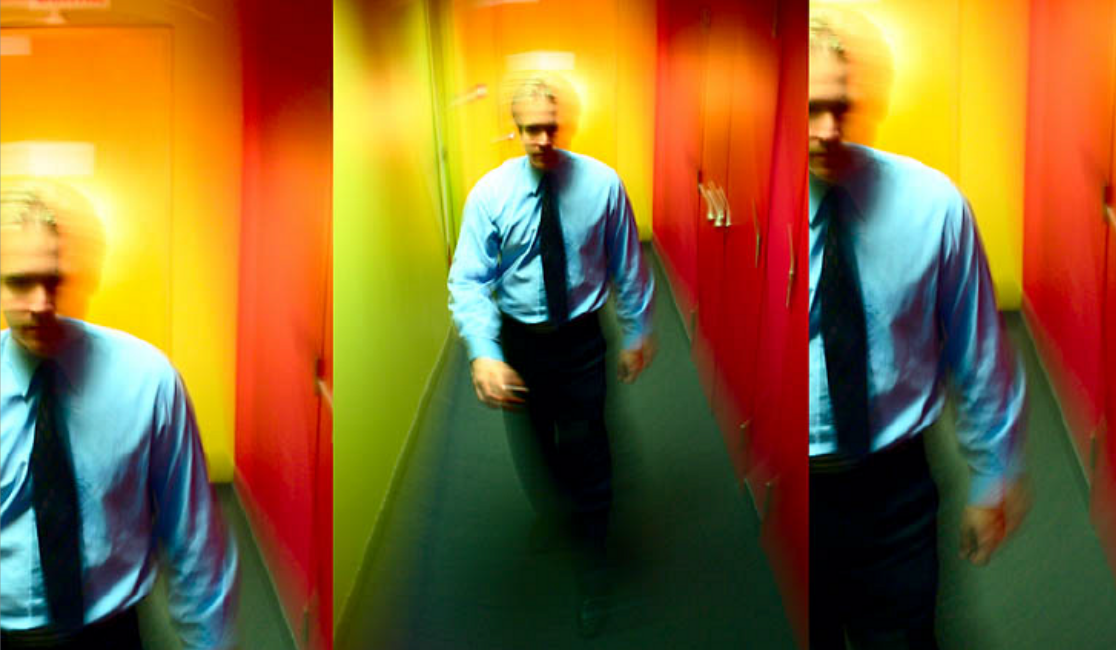
\includegraphics[width=0.9\textwidth]{figures/DDS.png}
    \end{tabular}
\end{frame}

\begin{frame}{Database, Data, and System Administration}
    \begin{itemize}
        \item Algunas organizaciones definen roles separados para los aspectos empresariales de los datos y los aspectos técnicos de los datos.
        \item Los aspectos de negocio de los datos están alineados con una disciplina conocida como administración de datos, mientras que los aspectos más técnicos son manejados por la administración de bases de datos. 
    \end{itemize}
\end{frame}

\begin{frame}{Database, Data, and System Administration}
    \begin{itemize}
        \item No todas las organizaciones tienen una función de administración de datos. De hecho, muchas organizaciones combinan la administración de datos en el rol de administración de bases de datos. 
        \item A veces, las organizaciones también dividen los aspectos técnicos de la gestión de datos, con el DBA siendo responsable de usar el DBMS y otro rol, conocido como administración del sistema o programación de sistemas, siendo responsable de instalar y actualizar el DBMS.
    \end{itemize}
\end{frame}

\begin{frame}{Data Administrator (DA) or Chief Data Officer (CDO)}
    \begin{itemize}
        \item No sobre tecnología, sobre datos y su significado en la organización...
        \item Responsable de reunir a la organización para tratar los datos como el activo corporativo que realmente es.
        \item Trata con metadatos y datos.
        \item Las organizaciones realmente preocupadas por la calidad, integridad y reutilización de los datos invariablemente implementarán y dotarán de personal la función de DA.
    \end{itemize}
\end{frame}

\begin{frame}{Metadata vs Data}
    \centering
    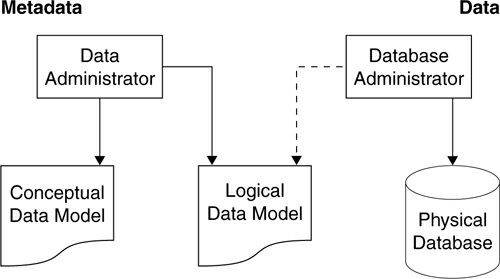
\includegraphics[width=0.75\textwidth]{figures/metadata2.png}
\end{frame}

\begin{frame}{System Administrator (SA)}
    \begin{itemize}
        \item Instalación y configuración de recursos informáticos.
        \item Tecnólogo puro.
        \item Sin responsabilidad por el diseño y soporte de la base de datos.
        \item Soporte de infraestructura.
        \item A veces llamado programador de sistemas.
    \end{itemize}
\end{frame}

\begin{frame}{Database Administrator (DBA)}
    \begin{itemize}
        \item Identifica y cataloga los datos requeridos por los usuarios empresariales.
        \item Produce modelos de datos conceptuales y lógicos para representar con precisión las relaciones entre los elementos de datos que ocurren dentro los procesos de negocio.
    \end{itemize}
\end{frame}

\begin{frame}{Database Administrator (DBA)}
    \begin{itemize}
        \item Produce un modelo de datos empresariales que incorpora todos los datos utilizados por todos los procesos de negocio de la organización.
        \item Configura las directivas de datos para la organización.
        \item Identifica propietarios, generadores y consumidores de datos.
        \item Establece estándares para el control y uso de datos.
    \end{itemize}
\end{frame}

\begin{frame}{Responsibilities}
    \centering
    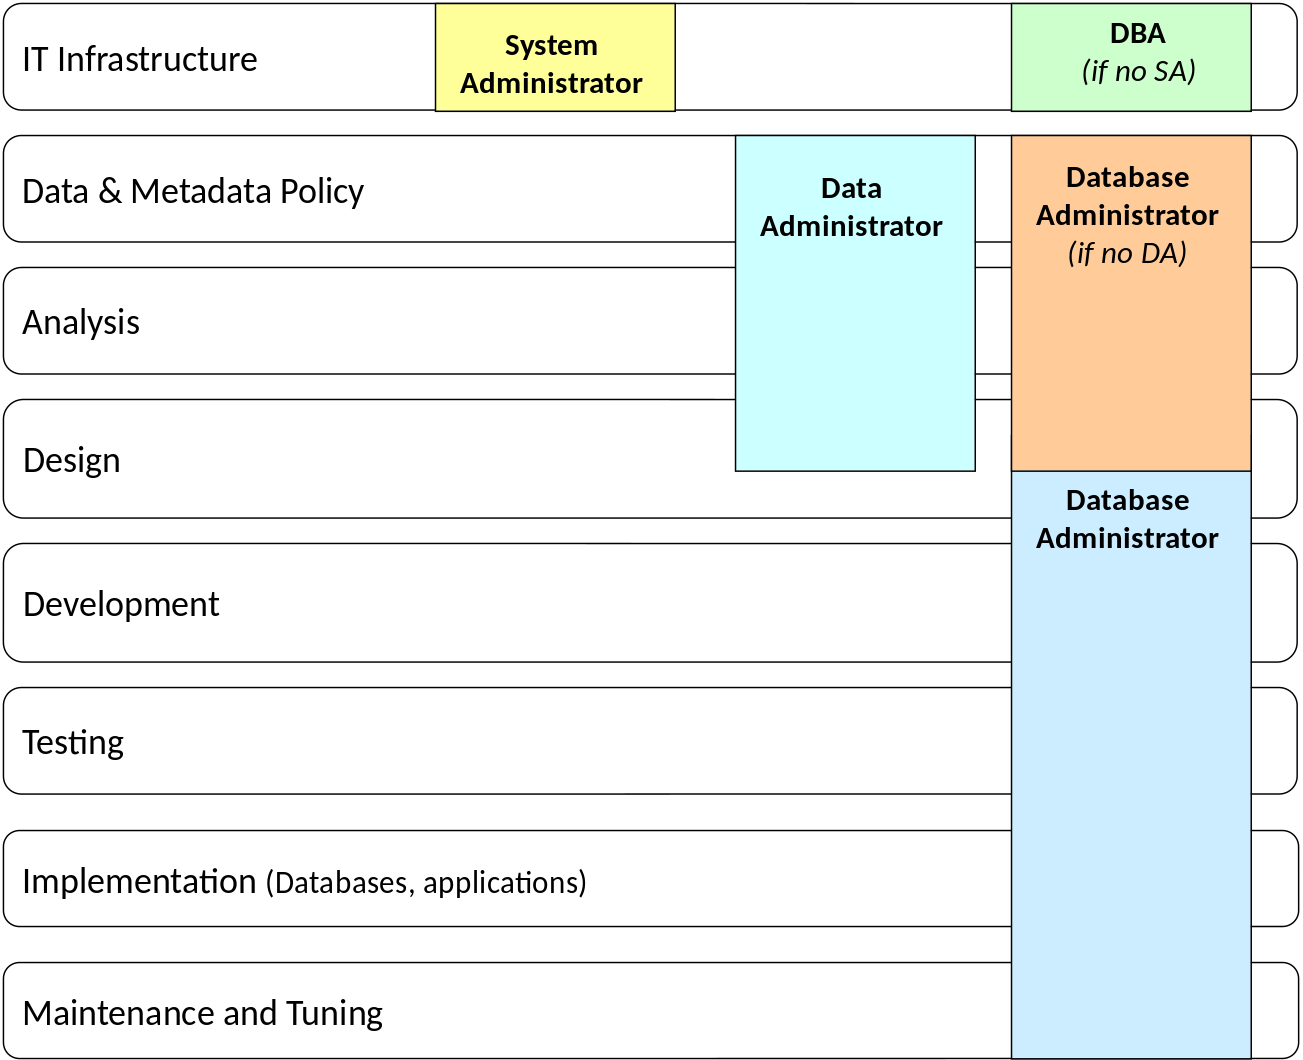
\includegraphics[width=0.9\textwidth]{figures/responsibilities.png}
\end{frame}

\begin{frame}{DBA Tasks}
    \centering
    Estas son las tareas de DBA necesarias para garantizar un entorno de base de datos óptimo para aplicaciones y usuarios:
    \begin{itemize}
        \item Crear el Ambiente o Entorno de las bases de datos.
        \item Diseñar las bases de datos.
        \item Diseñar aplicaciones que se conecten a las bases de datos.
        \item Revisar los diseños de las bases de datos.
        \item Liderar la gestión de cambios.
        \item Estar al tanto de la disponibilidad de los datos.
        \item Gestionar el desempeño.
        \begin{itemize}
            \item desempeño del sistema.
            \item desempeño de las bases de datos.
            \item desempeño de las aplicaciones asociadas.
        \end{itemize}
        \item Velar por la integridad de las bases de datos.
    \end{itemize}
\end{frame}

\begin{frame}{DBA Tasks}
    \centering
    Estas son las tareas de DBA necesarias para garantizar un entorno de base de datos óptimo para aplicaciones y usuarios:
    \begin{itemize}
        \item Estar al tanto de la seguridad de las bases de datos.
        \item Tolerancia a fallos, recuperación y copias de seguridad.
        \item Liderar planes de emergencia ante desastres.
        \item Gestión de almacenamiento.
        \item Mantenimiento y gestión de rutinas procedurales.
        \item Gestión de bases de datos distribuidas.
        \item Administración de Bodegas de Datos.
        \item Gerencia en las diferentes utilidades relacionadas a los SGBD instaladas.
        \item Conectividad a las diversas bases de datos.
        \item Cumplimiento normativo.
        \item Soft Skills!!!
    \end{itemize}
\end{frame}

\section{Types of DBA}

\begin{frame}{Types of DBAs}
    \begin{itemize}
        \item Los DBA se pueden centrar en:
        \begin{itemize}
            \item el diseño lógico...
            \item el diseño físico...
            \item la construcción de sistemas...
            \item el mantenimiento y ajuste de sistemas...
        \end{itemize}
        \item También existen DBAs especializados y DBAs de propósito general. Verdaderamente, el trabajo de DBA abarca muchos roles. 
    \end{itemize}
\end{frame}

\begin{frame}{Types of DBAs}
    \begin{itemize}
        \item Algunas organizaciones optan por dividir las responsabilidades de DBA en trabajos separados. 
        \item Por supuesto, esto ocurre con mayor frecuencia en organizaciones más grandes, porque las organizaciones más pequeñas a menudo no pueden permitirse el lujo de tener múltiples DBA especializados. 
        \item Otras empresas simplemente contratan DBA para realizar todas las tareas necesarias para diseñar, crear, documentar, ajustar y mantener los datos, bases de datos y sistemas de administración de bases de datos de la organización. 
    \end{itemize}
\end{frame}

\begin{frame}{Types of DBAs}
    \begin{itemize}
        \item Veamos algunos de los tipos más comunes de DBA:
        \begin{itemize}
            \item System DBA.
            \item Database Architect.
            \item Data Modeler.
            \item Application DBA.
            \item Task-Oriented DBA.
            \item Performance Analyst.
            \item Data Warehouse Administrator.
        \end{itemize}
    \end{itemize}
\end{frame}

\begin{frame}{Database Architect}
    \begin{itemize}
        \item Creación de un modelo de datos lógico (si no existe una posición de DA o modelador de datos).
        \item Traducción de modelos de datos lógicos en diseños de bases de datos físicas.
        \item Implementación de bases de datos eficientes, lo que incluye:
        \begin{itemize}
            \item las características físicas, 
            \item el diseño de índices y 
            \item la asignación de los datos a dispositivos de almacenamiento físico.
        \end{itemize}
        \item Análisis de los requisitos de acceso y modificación de datos para garantizar consultas SQL eficientes.
        \item Creación de estrategias de backup y recuperación para nuevas bases de datos.
    \end{itemize}
\end{frame}

\begin{frame}{Data Warehouse Administrator}
    \begin{itemize}
        \item Experiencia con inteligencia empresarial, análisis de datos, consultas y herramientas de informes.
        \item Diseño de base de datos para acceso de solo lectura.
        \item Problemas de diseño de almacenamiento de datos, como el esquema en estrella.
        \item Tecnologías de almacenamiento de datos como OLAP (incluidos ROLAP, MOLAP y HOLAP).
        \item Habilidades de transformación y conversión de datos (ETL jobs).
        \item Una comprensión de los problemas de calidad de los datos.
        \item Experiencia con formatos de datos para carga y descarga de datos.
        \item Implementación y administración de middleware.
    \end{itemize}
\end{frame}

\begin{frame}{System DBA}
    \begin{itemize}
        \item Instalación de nuevas versiones de DBMS y aplicación de correcciones de mantenimiento proporcionadas por el proveedor de DBMS.
        \item Configuración y ajuste de los parámetros del sistema.
        \item Ajuste del sistema operativo, la red y los procesadores de transacciones que funcionen con el DBMS.
        \item Garantizar el almacenamiento adecuado para el DBMS.
        \item Permitir que el DBMS funcione con dispositivos de almacenamiento y software de administración de almacenamiento.
        \item Interfaz con cualquier otra tecnología requerida por las aplicaciones de base de datos.
        \item Instalación de herramientas y utilidades de DBA.
    \end{itemize}
\end{frame}

\begin{frame}{Data Modeler}
    \begin{alertblock}{Nota}
        Cuando el rol de DA no está definido o dotado de personal, puede haber un rol de modelador de datos definido. Un modelador de datos suele ser responsable de un subconjunto de las responsabilidades del DA.
    \end{alertblock}
    \begin{itemize}
        \item La recopilación de requisitos de datos para proyectos de desarrollo.
        \item Análisis de los requisitos de datos.
        \item Diseño de modelos de datos conceptuales y lógicos basados en proyectos.
        \item Creación de un modelo de datos corporativo y mantenimiento y actualización de dicho modelo.
        \item Trabajar con los DBA para garantizar que tengan una sólida comprensión de los modelos de datos.
    \end{itemize}
\end{frame}

\begin{frame}{Task-Oriented DBAs}
    DBA que se centran en un subconjunto limitado de tareas de administración de bases de datos.  Por ejemplo:
    \begin{itemize}
        \item DBAs de Backup y Recuperación.
        \item Diseñador de bases de datos.
        \item Analistas de rendimiento.
    \end{itemize}
\end{frame}

\begin{frame}{Application DBA}
    \begin{itemize}
        \item En contraste directo con el DBA del sistema está el DBA de aplicación. 
        \item Los DBA de aplicaciones se centran en el diseño de bases de datos y el soporte y administración continuos de bases de datos para una aplicación o aplicaciones específicas.
        \item El DBA de aplicaciones es un experto en escribir y depurar SQL complejo.
        \item Comprende las mejores formas de incorporar solicitudes de base de datos en los programas de aplicación. 
    \end{itemize}
\end{frame}

\begin{frame}{Application DBA}
    \begin{itemize}
        \item El DBA de la aplicación también debe ser capaz de realizar:
        \begin{itemize}
            \item la administración de cambios de la base de datos, 
            \item el ajuste del rendimiento y 
            \item la mayoría de los demás roles del DBA. 
        \end{itemize}
    \end{itemize}
    \begin{alertblock}{Nota}
        La diferencia está en el enfoque a aplicaciones y no tanto a la implementación general de DBMS; No se centra en el entorno de base de datos, sino más en el subconjunto específico de aplicaciones.
    \end{alertblock}
\end{frame}

\begin{frame}{Focus of the Application DBA}
    \centering
    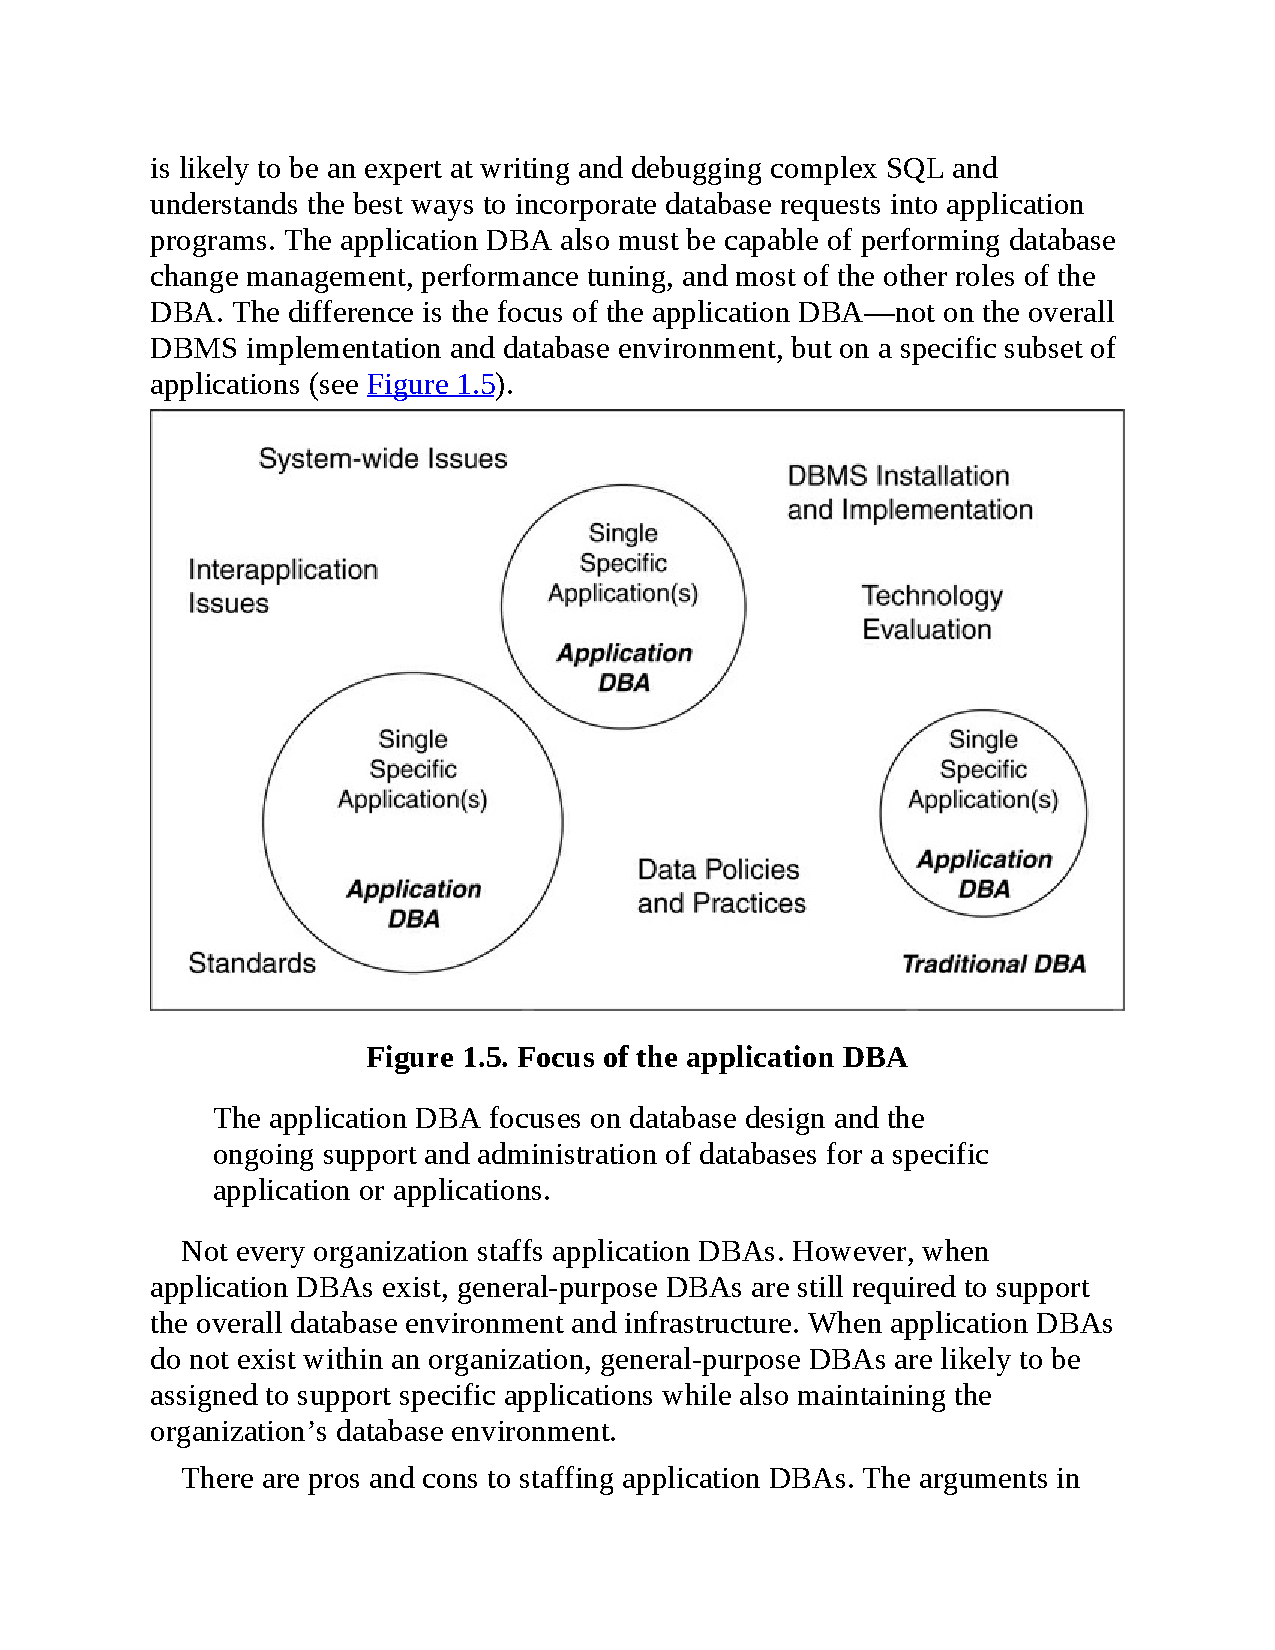
\includegraphics[width=\textwidth, trim={2.55cm 10.60cm 2.55cm 6.80cm}, clip]{figures/app_dba}
\end{frame}

\begin{frame}{DBA Reporting Structures}
    Typical DBA reporting structure:\\
    \vspace{5mm}
    \centering
    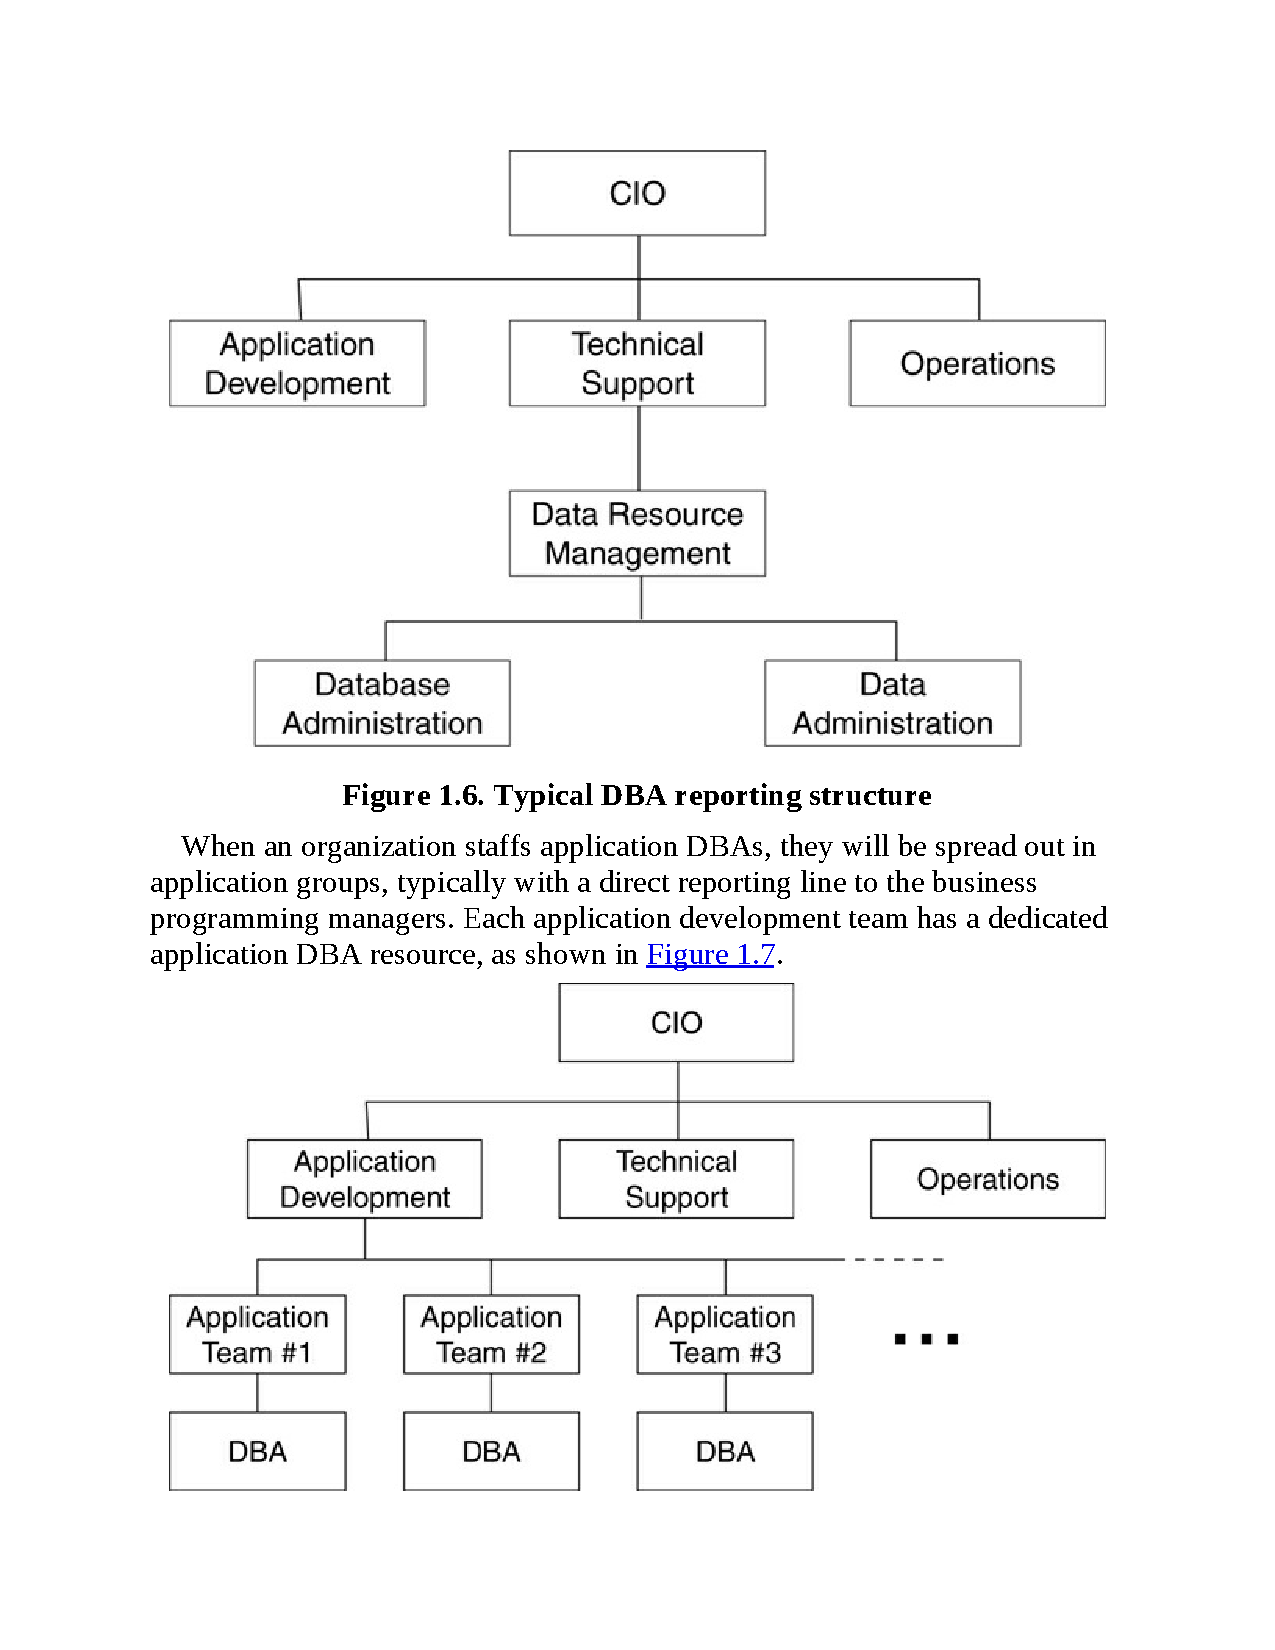
\includegraphics[width=0.8\textwidth, trim={2.55cm 14.80cm 2.55cm 2.50cm}, clip]{figures/dba_reporting1}
\end{frame}

\begin{frame}{DBA Reporting Structures}
    Application DBA reporting structure:\\
    \vspace{5mm}
    \centering
    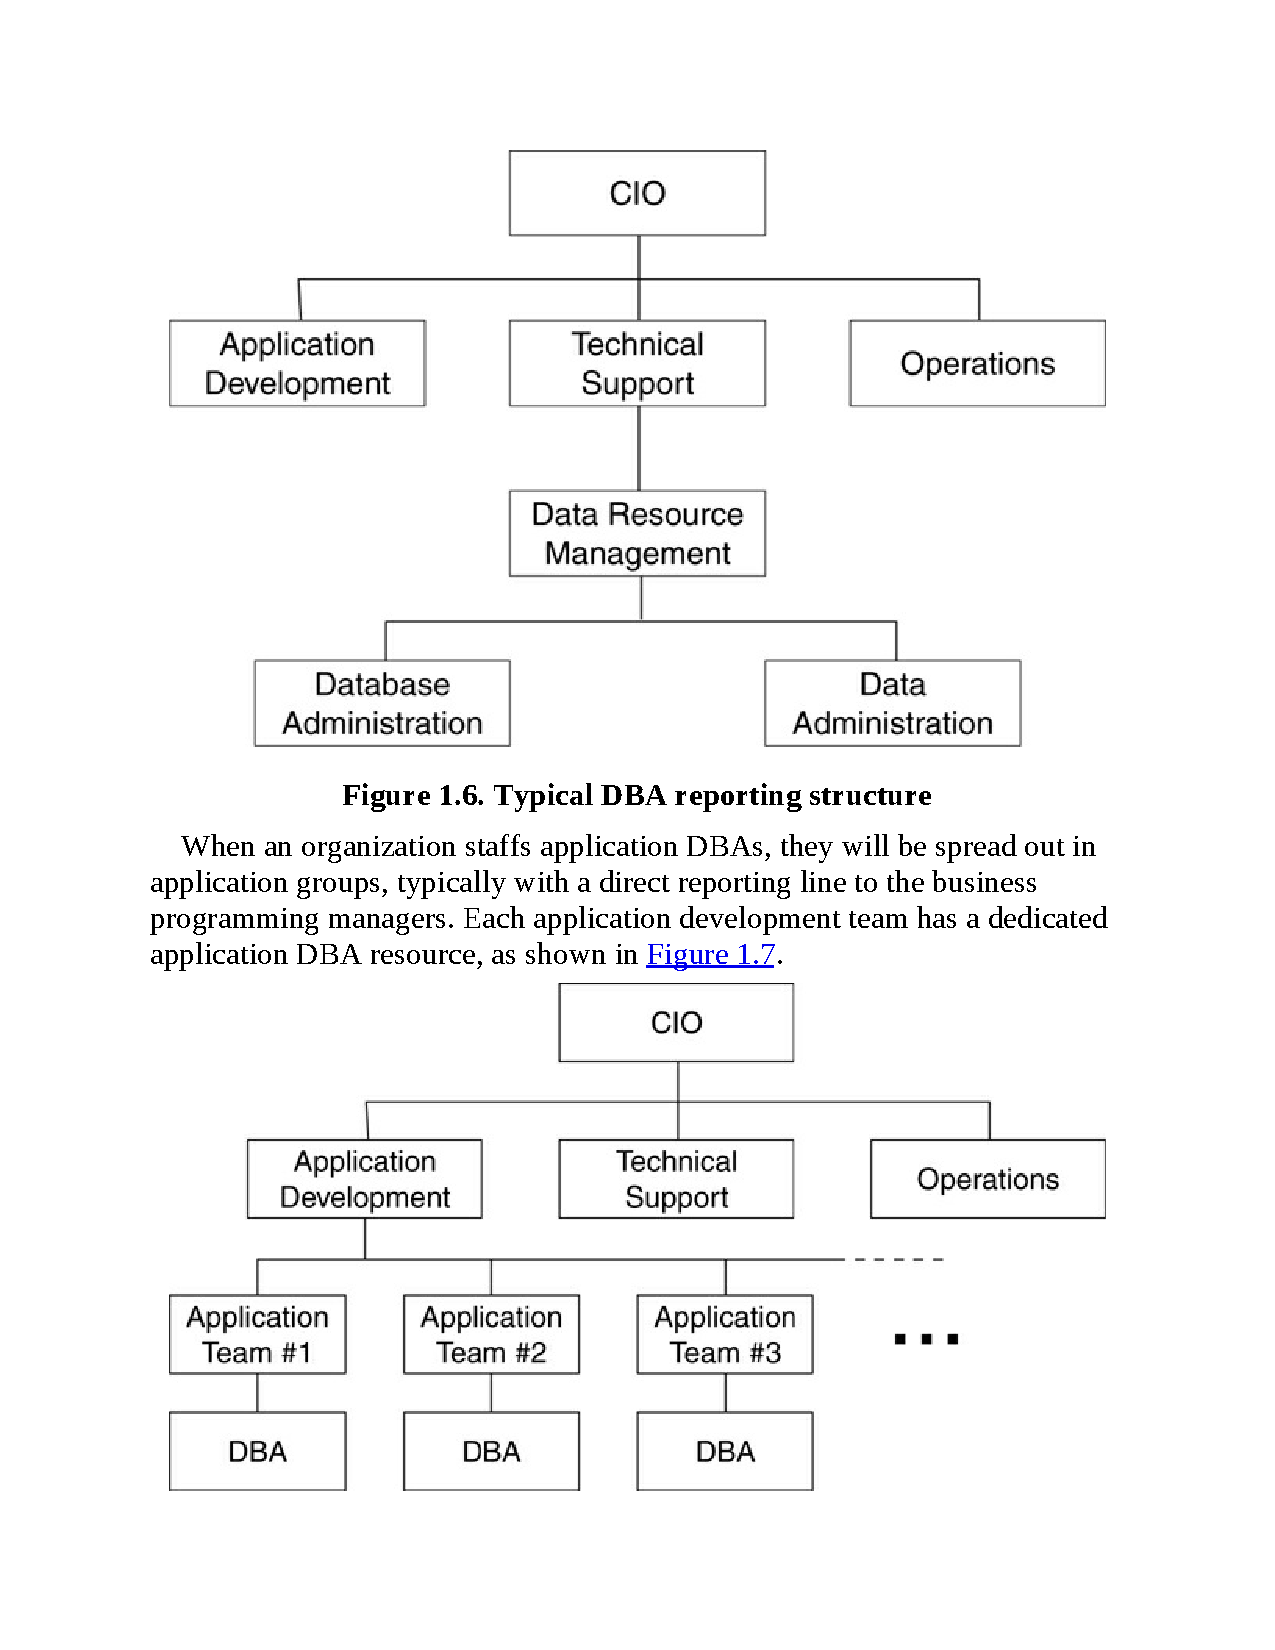
\includegraphics[width=0.9\textwidth, trim={2.55cm 2.60cm 2.55cm 16.50cm}, clip]{figures/dba_reporting1}
\end{frame}

\begin{frame}{DBA Reporting Structures}
    Recommended DBA reporting structure:\\
    \vspace{5mm}
    \centering
    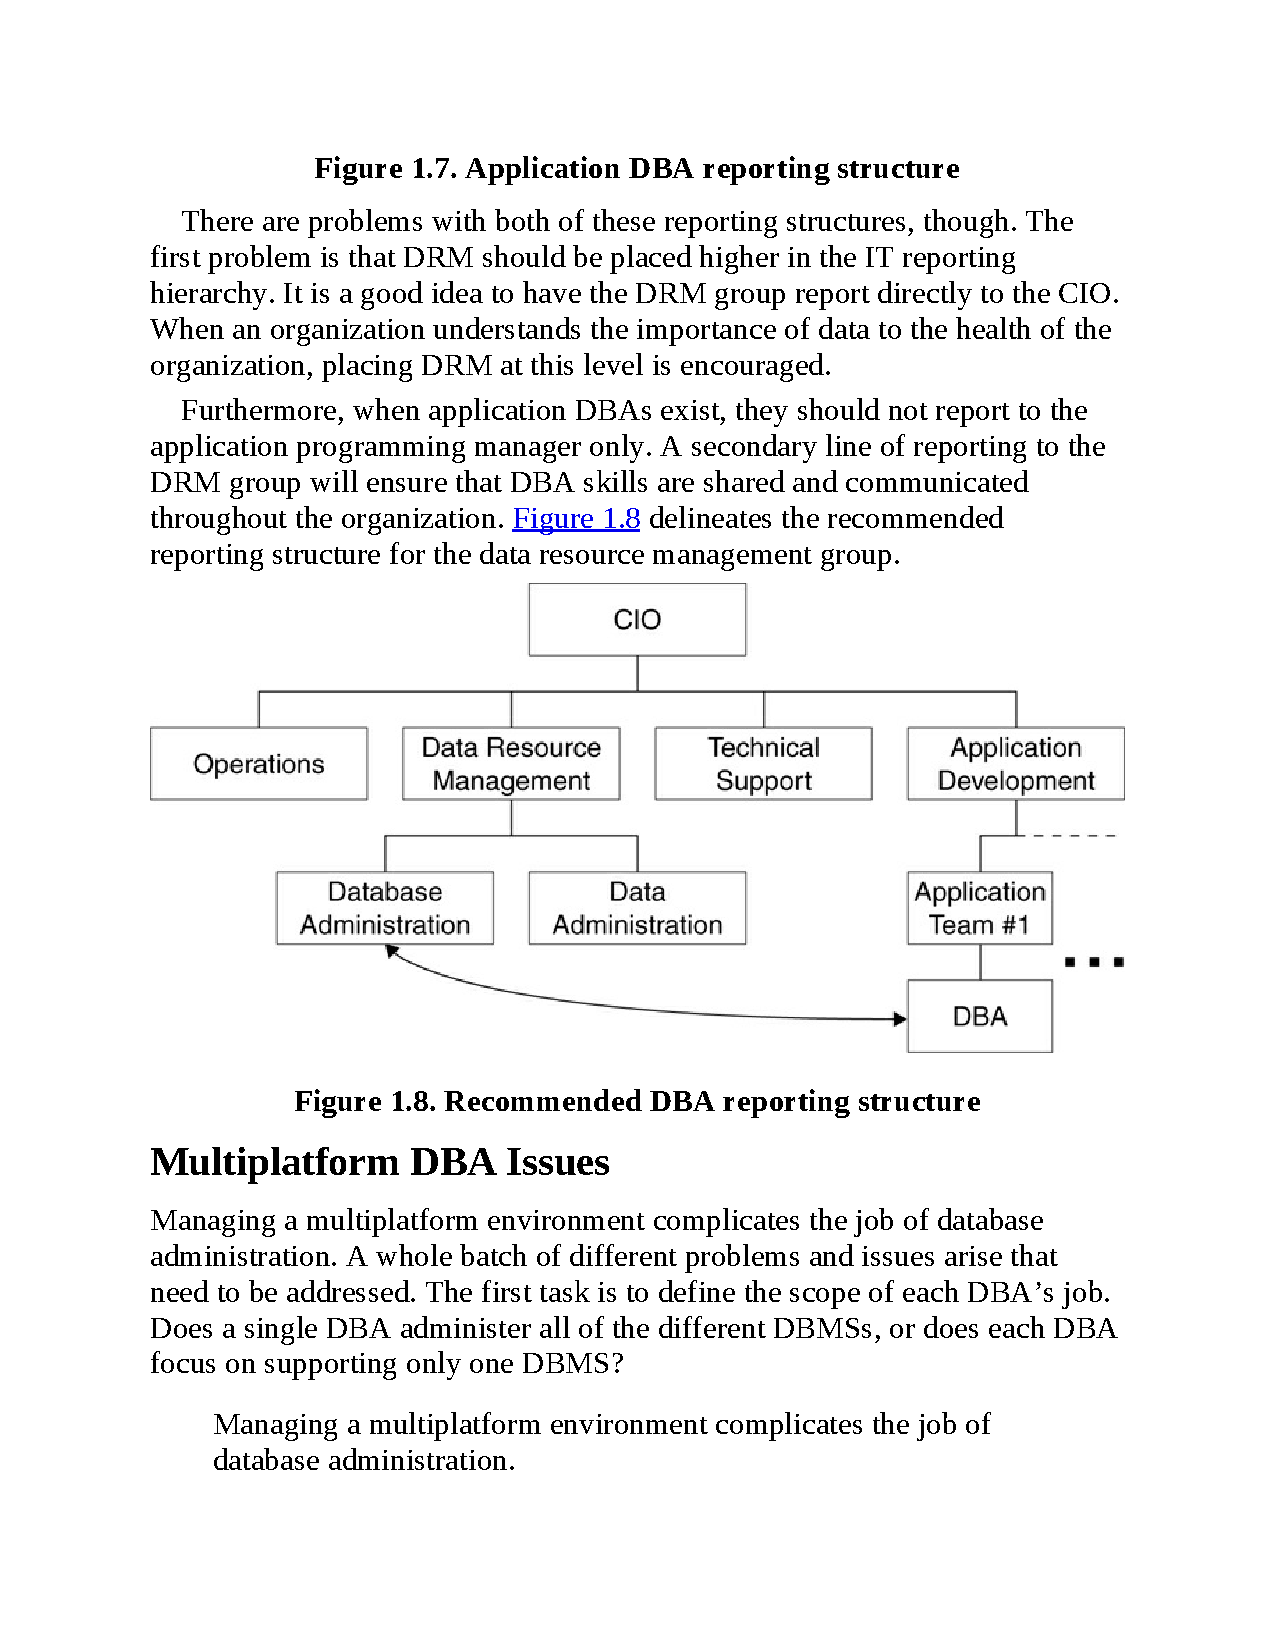
\includegraphics[width=0.9\textwidth, trim={2.55cm 9.60cm 2.55cm 9.80cm}, clip]{figures/dba_reporting2}
\end{frame}

\begin{frame}{Production versus Test}
    \begin{itemize}
        \item At least two separate environments must be created and supported for a quality database implementation: production and test (or development).
        \item It is necessary to completely separate the test environment from the production environment to ensure the integrity and performance of operational work.
    \end{itemize}
    \begin{alertblock}{Note}
        Separating the test and production environments ensures the integrity and performance of operational work.
    \end{alertblock}
\end{frame}

\begin{frame}{Establishing multiple database environments}
    \centering
    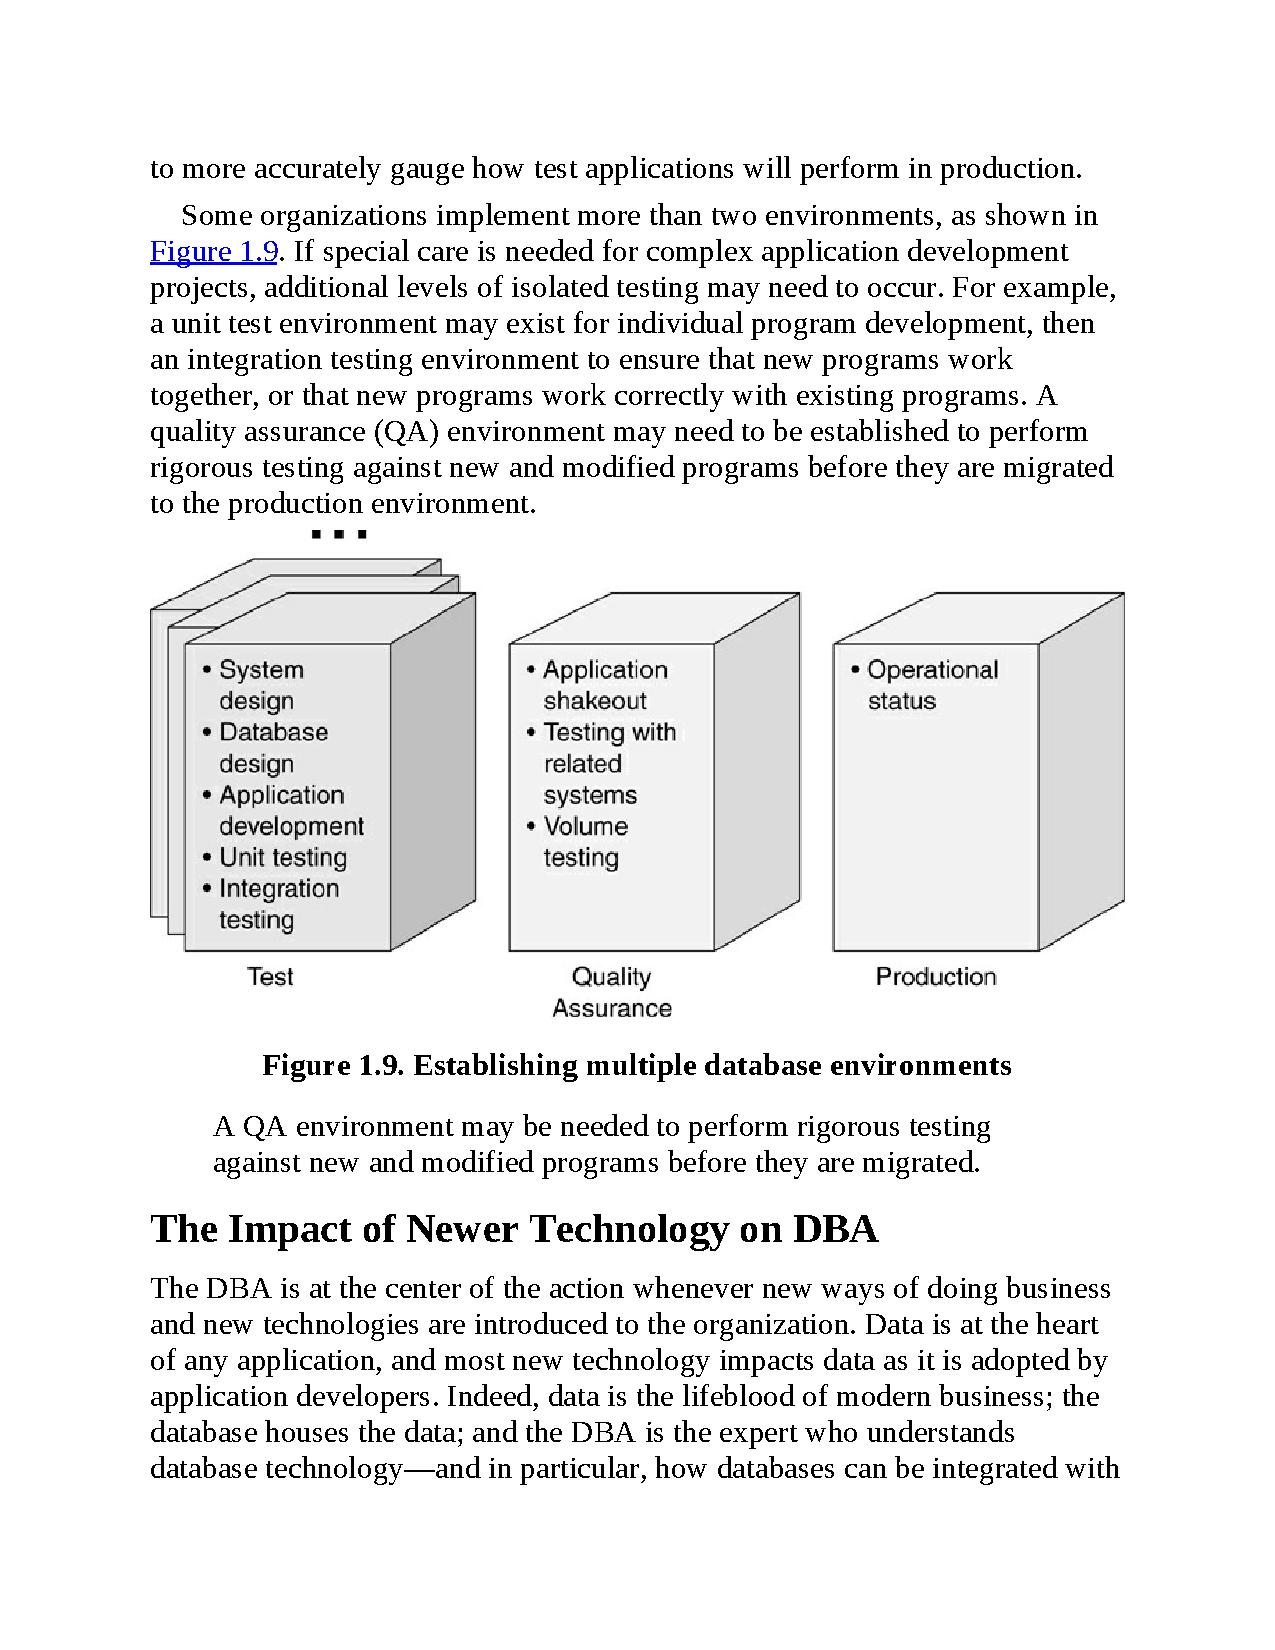
\includegraphics[width=\textwidth, trim={2.50cm 10.20cm 2.50cm 9.40cm}, clip]{figures/dba_test}
\end{frame}

\section{Procedural DBAs: Managing Database Logic}

\begin{frame}{Procedural DBAs: Managing Database Logic}
    \small
    \centering
    \begin{tabular}{ l l c c}
        \toprule
        Object & Definition & Executed & How \\
        type & & & \\
        \midrule
        Stored  & Program logic executed on & By request & Explicit \\
        procedures & the database server. & & \\
        Triggers & Event-driven procedures & Automatic & Implicit \\
        & attached to database tables. & & \\
        UDFs & Program logic extending & By request & Explicit \\
        & SQL functionality. & SQL & \\
        \bottomrule
    \end{tabular}
\end{frame}

\begin{frame}{Procedural DBAs: Managing Database Logic}
    \footnotesize
    \centering
    \begin{tabular}{ l l }
        \toprule
        Object & Level of Procedular DBA Involvement \\
        type & \\
        \midrule
        Stored  & Not likely to actually write stored procedures; \\
        procedures & must review all code before procedures migration to production; \\
        & should communicate availability and promote reuse. \\
        Triggers & Likely to actually write, test, and debug triggers; \\
        &must communicate deployment to ensure application awareness. \\
        UDFs & Not likely to actually write user-defined functions; \\
        & should work closely with the development team; \\
        & must review all code before migration to production; \\
        & must communicate availability and promote reuse. \\
        \bottomrule
    \end{tabular}
\end{frame}

\begin{frame}{Procedural DBA duties}
    \centering
    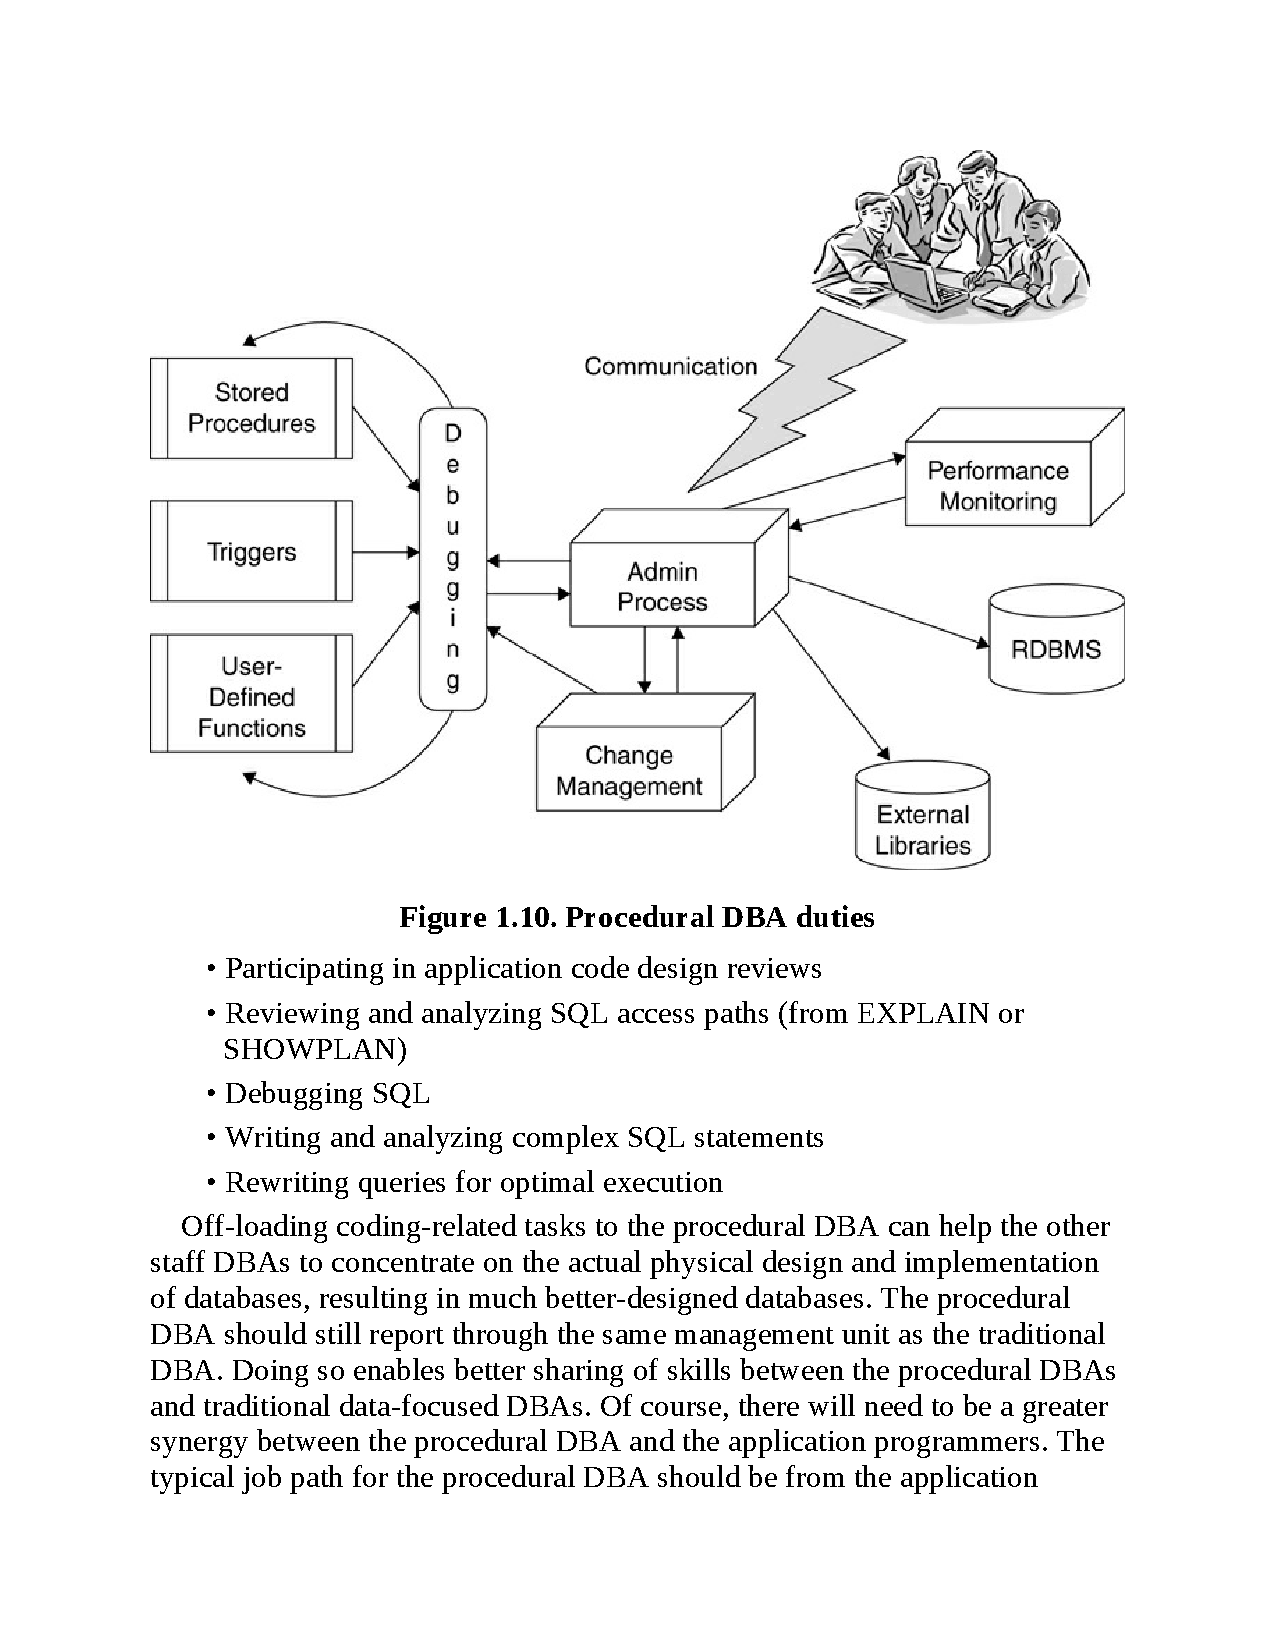
\includegraphics[width=\textwidth, trim={2.50cm 13.00cm 2.50cm 2.40cm}, clip]{figures/dba_duties}
\end{frame}

\section{The Internet: from DBA to eDBA}

\begin{frame}{The Internet: from DBA to eDBA}
    \begin{itemize}
        \item \textbf{Internet's Impact on Business Processes:} Companies continue adapting their processes to align with e-commerce, affecting database administration practices.
        \item \textbf{E-Business Requires Constant Availability:} Online businesses must operate 24/7 since customers expect full functionality at all times, and competition is just a click away.
        \item \textbf{High Demands on DBAs:} E-businesses require DBAs to integrate web technologies with traditional IT services, increasing their workload and responsibilities.
        \item \textbf{The Role of an eDBA:} An eDBA (electronic DBA) needs both traditional DBA skills and specialized expertise in managing Internet-enabled applications and databases.
    \end{itemize}
\end{frame}

\begin{frame}{Complex Infrastructure Management}
    \centering
    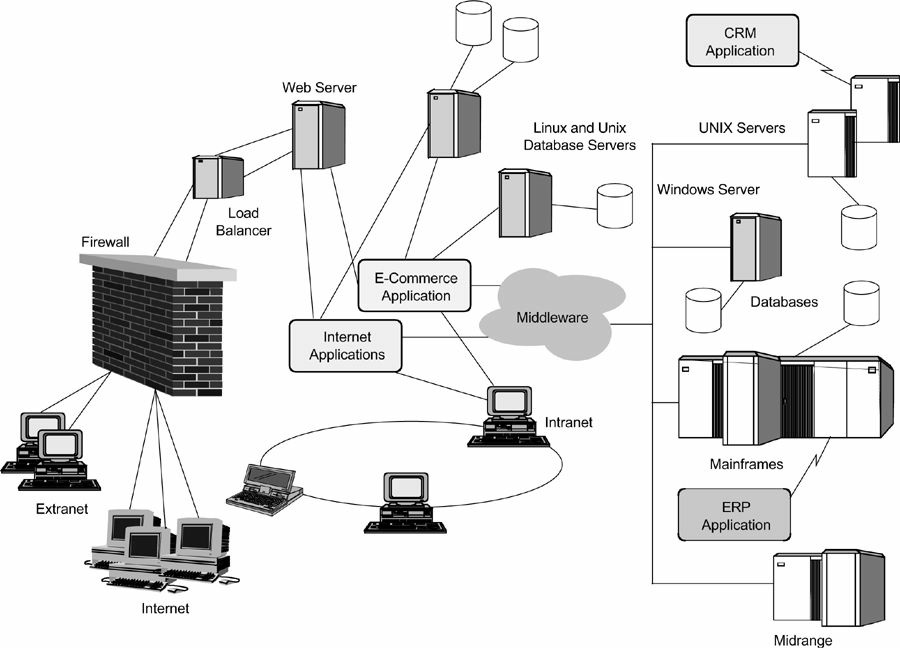
\includegraphics[width=\textwidth]{figures/dba_cloud.png}
\end{frame}

\begin{frame}{}
    \centering
    \Huge End of Chapter 1.
\end{frame}

\section*{Takeaways}

\begin{frame}{TDT5FTOTTC}
    \centering
    
\includegraphics[width=0.45\textwidth]{figures/td.jpg}\\
    \href{https://en.wikipedia.org/wiki/Tim_Duncan}{Tim Duncan in Wikipedia.}
\end{frame}

% Tim Duncan's Top 5 Fundamental Takeaways of the Today's Class
\begin{frame}{TDT5FTOTTC}
    \centering
    
\includegraphics[width=0.75\textwidth]{figures/tim.png}
\end{frame}

\begin{frame}{Top 5 Fundamental Takeaways}
    \begin{enumerate} \pause
        \item[5] \textbf{DBAs Are Essential but Often Misunderstood} – Every organization using databases needs a DBA, but their role is frequently undervalued despite its critical importance.\pause
        \item[4] \textbf{Balancing Stability and Change is Key} – DBAs must manage database stability while accommodating business changes, often navigating tensions with developers.\pause
        \item[3] \textbf{DBA Responsibilities Go Beyond Design} – Their role includes performance monitoring, security enforcement, backup and recovery, system upgrades, and compliance.\pause
        \item[2] \textbf{Collaboration is Crucial} – DBAs work closely with Data Administrators (DAs) on data policies and modeling and System Administrators (SAs) on IT infrastructure.\pause
        \item[1] \textbf{Protecting Data is the Core Responsibility} – DBAs ensure data integrity, security, availability, and performance, making databases reliable and efficient.
    \end{enumerate}
\end{frame}

\begin{frame}{Database Administration: The Complete Guide to Practices and Procedures.}
    \centering
    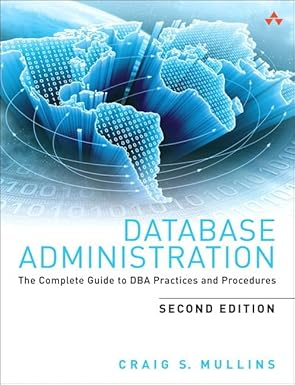
\includegraphics[width=0.3\textwidth]{figures/book_cover.jpg} \\
    \vspace{5mm}
    {
        \tiny
        Content has been extracted from \textit{Database Administration: The Complete Guide to Practices and Procedures.}, Second Edition, by Craig S. Mullin. Addison-Wesley Professional. 2012.\\
        Visit \url{https://www.craigsmullins.com/books.htm}.\\
    }
\end{frame}

\end{document}
